\documentclass[
../../NLP4W_Summary.tex,
]
{subfiles}
    
\externaldocument[ext:]{../../NLP4W_Summary.tex}
% Set Graphics Path, so pictures load correctly
\graphicspath{{../../}}

\begin{document}
\section{Text Classification}
Text classification is an important part of NLP4Web. It has many applications and it's especially important to classify text to improve the date of the models.

\begin{defbox}
    [Examples of Text Classification]
    \begin{itemize}
        \item Spam Detection
        \item Sentiment Analysis
        \item Topic Labeling
        \item Age/Gender Identification
        \item Authorship Identification
        \item Language Identification
    \end{itemize}
\end{defbox}

Some approaches to text classification are:

\begin{defbox}
    [Approaches to Text Classification]
    \begin{itemize}
        \item Rule-Based
        \begin{itemize}
            \item Rules are "handcrafted" and human comprehensible
            \item As such precision can be high
            \item However it might also be very expensive to build and maintain as it needs to cover a lot of cases and handle changing languages
        \end{itemize}
        \item Supervised Learning
        \begin{itemize}
            \item Processes by which tagged/labeled data is picked and fed into an algorithm that then builds a model capaable of approximating text
            \item Can be human comprehensible - but doesn't need to be
            \item Easier to meaintain and fairly accurate
            \item Needs a lot of data
        \end{itemize}
        \item Unsupervised Learning (Deep Learning)
    \end{itemize}
\end{defbox}

\subsection{Naive Bayes Classifier}
Naive Bayes is an algorithm for text classification. It is based on conditional Probabilites and Bayes Rule. 

\begin{defbox}
    [Conditional Probabilites]
    \textit{The probability that something will happen, given that else has already happened}
    \begin{itemize}
        \item Assume \textbf{Outcome O} and \textbf{Evidence E}
        \item Then 
        \begin{itemize}
            \item $P(O,E)$ describes the probability of both O and E occuring\\
            \rightarrow \inlmathbox{$P(O,E) = P(O) \times P(E|O)$}
            \item $P(O)$ describes the probability of O occuring\\ 
            \rightarrow \inlmathbox{$P(O) = \dfrac{P(O,E)}{P(E|O)}$}
            \item $P(E|O)$ describes the probability of E given O\\
            \rightarrow \inlmathbox{$P(E|O) = \dfrac{P(E,O)}{P(O)}$}
        \end{itemize}
    \end{itemize}
\end{defbox}

\begin{defbox}
    [Bayes Rule]
    Bayes Rule conceptually describes a way to go from $P(E|O)$ to $P(O|E)$

    This can be done with the formula:\\
    \begin{center}
        \begin{smallmathbox*}
            $P(O|E) = \dfrac{P(E|O) \times P(O)}{P(E)}$
        \end{smallmathbox*}
    \end{center}
\end{defbox}

Unfortunately, Bayes rule only works for one piece of evidence at a time. For efficient text classification this is not enough, which is what \textbf{Naive Bayes} is for, as it can predict the outcome given multiple pieces of evidence.

\begin{defbox}
    [Naive Bayes Classifier]
    Naive Bayes treats each piece of evidence as independent, which makes it easier to calculate (hence why \textit{naive})
    \begin{center}
        \begin{smallmathbox*}
            $P(O|E1,\ldots,E_n) = \dfrac{P(E_1|O) \times P(E_2|O) \times \ldots \times P(E_n|O) \times P(O)}{P(E_1, E_2, \ldots, E_n)}$
        \end{smallmathbox*}
        
        Easier to remember:

        \begin{smallmathbox*}
            $P(\text{outcome}|\text{evidence}) = \dfrac{P(\text{Likelihood of Evidence}) \times \text{Prior probability of outcome}}{P(\text{Evidence})}$
        \end{smallmathbox*}
    \end{center}
\end{defbox}

\begin{defbox}
    [Multinomial Naive Bayes Model]
    \begin{center}
        \begin{smallmathbox*}
            \shortstack{
            $P(c|d) \varpropto P(c) \prod\limits_{1\leq k \leq n_d} P(t_k | c)$ \\
            with Posterior Probability $P(c|d)$ and Prior Probability $P(c)$
            }
        \end{smallmathbox*}
    \end{center}
    The probability of document \textbf{d} belonging to class \textbf{c} is proportional to the product of the probabilities of terms \textbf{t} belonging to \textbf{c} and to the class prior \textbf{P(c)}

    \begin{center}
        \begin{smallmathbox*}
            $c_{\text{map}} = \mathop{\arg\max}\limits_{c \in C}\space \hat{P}(c|d) = \mathop{\arg\max}\limits_{c \in C} \space \hat{P}(c) \prod\limits_{1\leq k \leq n_d} \hat{P}(t_k | c)$ 
        \end{smallmathbox*}
    \end{center}
    The best class \textbf{c} for a document \textbf{d} is found by selecting the class for which the maximum a posteriori (map) probability is maximal.
\end{defbox}

So overall Naive Bayes provides us with a method to determine the most probable hypothesis given the data. This is based on probability calculation, therefore no training of a model is necessary.

However, Naive Bayes fails if the independence assumption is violated too much. Meaning that identical or overlapping features pose a problem, which necessitates proper feature selection.

\newpage
\subsection{Hidden Markov Models (HMM)}

As many problems in NLP do have overlapping or identical data, Naive Bayes cannot always be relied upon. 

\subsubsection{Sequence Labeling through Classification}

Many NLP problems can be viewed as sequence labeling. Hereby each token in a sequence is assigned a label. These labels are not independent of each other but depend on the other tokens in the sequence, especially their neighbors. One example of this is part of speech tagging.

This can be done using different techniques, the simplest being classification. Hereby tokens are identified by the token itself (using lexical knowledge) but also by their neighbors. This "rolling window" will then go through the whole sequence classifying each token.

This does not give us a good solution, as the classification of the surrounding tokens are more important than the token itself for classification. To improve on this, we can now go through the sequence again using the same approach but this time using the classifiers itself as the inputs. This can be done forwards or backwards, which might result in different classifications.

This yields some problems though. As forwards and backwards can yield different results, it's hard to tell which classifications are correct or wrong and which should be adopted. This uncertainty cannot be solved in this method.

\subsubsection{Hidden Markov Model Concept}

A Hidden Markow Model (HMM) is a statistical model of hidden, stochastic state transitions with observable, stochastic output. 

\begin{defbox}
    [Hidden Markov Model Key Characteristics]
    \begin{itemize}
        \item Fixed set of states: At each time the model is in exactly one of these states
        \item State transition probabilities: The probability of transitioning from one state to another. The starting state can be fixed or random.
        \item Fixed set of possible outputs
        \item Distribution of probabilities for each possible output (Emission probabilities)
    \end{itemize}
    The HMMs purpose is to answer the question: \textbf{For an observed output sequence, what is the (hidden) state sequence that has the highest probability to produce this output?}
\end{defbox}

One example of such a model is the following. Here the states are representative of the moods of Darth Vader (wearing a mask, therefore hidden) and the emissions are whether or not he blows up a planet on this day. S represents the starting mood. (Not Blown up (NB), Blown up (BU), Happy (H), Angry (A), Neutral (N))

\begin{figure}[htp]
    \centering
    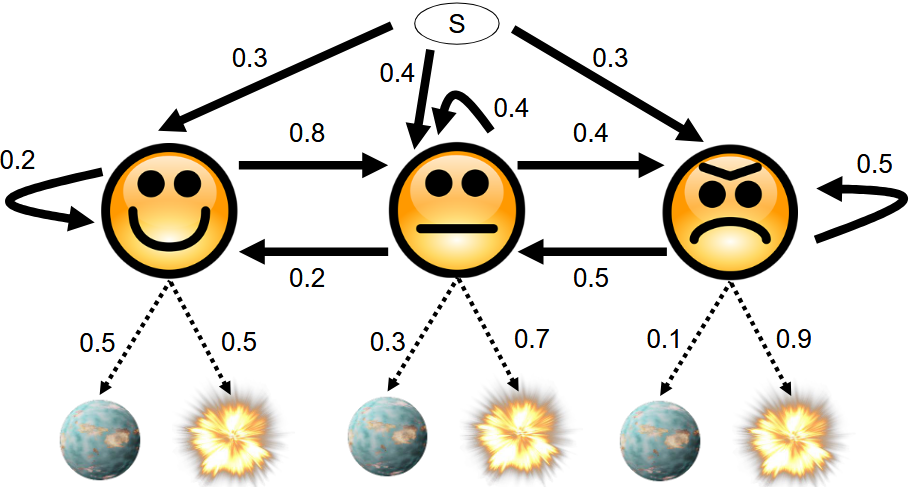
\includegraphics[scale=0.35]{Pics/HMMExampleVader.png}
\end{figure}

Now, we can observe whether or not he blows up a planet on a given day. But what is the most probable sequence of moods for a given sequence of emission? 

Assume the following sequence of emissions: Not Blown Up, Blown up, Blown up. What is the probability that this sequence coincides with the following sequence of moods: Angry, Neutral, Angry?

For this we need to consider the transition and emission probabilities on each day. 

For the first day this means, that we need the transition probability from starting point to angry (0.3) and the emission probability of Not Blown up for Angry (0.1). The joint probability on the first day is then given by \inlmathbox{$P(\text{NB}, \text{A})= 0.3 \cdot 0.1 = 0.03$}

For the second day we need the transition probability from angry to neautral (0.5) and the emission probability of Blown up for Neutral (0.7). The joint probability on the second day is then given by \inlmathbox{$P(\text{BU}, \text{N}) = 0.5 \cdot 0.7 = 0.35$} Additionally this gives us the probability for the sequence \inlmathbox{$P(\{\text{A} \rightarrow \text{N}\}|\{\text{NB}, \text{BU}\}) = 0.03 \cdot 0.35 = 0.0105$}

For the third day we need the transition probability from neutral to angry (0.4) and the emission probability of Blown up for Angry (0.9). The probability for the joint probability on the third day is then given by \inlmathbox[mathbox]{$P(\text{BU}, \text{A}) = 0.4 \cdot 0.9 = 0.36$}. \\This also gives us the probability for the sequence \inlmathbox{$P(\{\text{A} \rightarrow \text{N} \rightarrow \text{A}\} | \{\text{NB}, \text{BU}, \text{BU}\}) = 0.03 \cdot 0.35 \cdot 0.36 = 0.00378$}

\subsubsection{Hidden Markov Model in NLP}
We can apply this model to POS tagging. The sequence of qords are the observable emissions, while the POS tags are the hidden states. 
We also require the transition probabilities between the states, the initial probabilities and the emission probabilities. 

These probability are usually estimated by counting on a tagged training corpus. Hereby the following probabilities are given:
\begin{center}
    \begin{smallmathbox}
        [Transition probabilities]
        \shortstack{
            $P(t_i | t_{i-1}) = \dfrac{C(t_{i-1}, t_i)}{C(t_{i-1})}$ \\
            $ = \dfrac{\text{How often the first tag is followed by the second tag}}{\text{How often the first tag occured in the labeled corpus}}$
        }
    \end{smallmathbox}
    
    \begin{smallmathbox}
        [Emission probabilities]
        \shortstack{
            $P(w_i | t_i) = \dfrac{C(t_i, w_i)}{C(t_i)}$ \\
            $ = \dfrac{\text{How often the word was associated with the tag in the labeled corpus}}{\text{How often the first tag occured in the labeled corpus}}$
        }
    \end{smallmathbox}
\end{center}

\begin{figure}
    [htp]
    \centering
    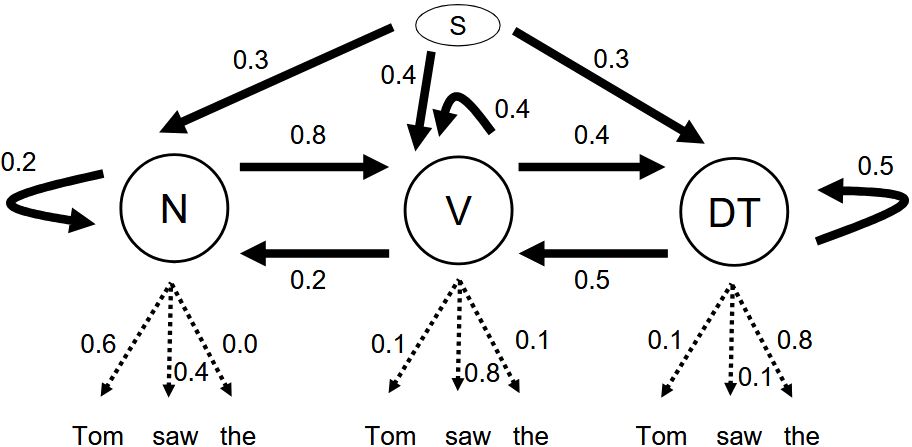
\includegraphics[scale=0.45]{Pics/HMMExampleNLP.png}
    \caption{Example HMM for Sequence Tagging}
\end{figure}

\begin{center}
    \begin{smallmathbox*}
        \shortstack{
            $\hat{t}^n_1 = \mathop{\arg\max}\limits_{t_1^n}\space P(t_1^n | w_1^n) \approx \mathop{\arg\max}\limits_{t_1^n}\space \prod\limits_{i=1}^n \underbrace{P(w_i | t_i)}_{\text{Emission}}\space \underbrace{P(t_i | t_{i-1})}_{\text{Transition}}$ \\ $\hat{t}^n_1$ is the most likely state sequence given an output sequence
        }
    \end{smallmathbox*}
\end{center}

How do we calculate this? One solution would be brute force search by enumerating all possible sequences of states. This gives us a complexity of $O(s^m)$ where $s$ is the number of states and $m$ the length of the sequence. 

A better solution would be the Viterbi algorithm, which uses a Dynamic Programming approach. This gives us a complexity of $O(ms^2)$.

\subsection{Viterbi Algorithm}
Viterbis algorithm works by calculating the joint probability for each tag for each word. It uses the principles of HMM to get the necessary probabilities. 

After it has done that for each word it iterates backwards through the input again and finds the most probable tag for the word. 

\begin{figure}[htp]
    \centering
    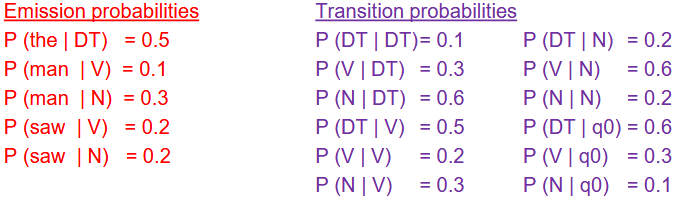
\includegraphics[scale=0.5]{Pics/ViterbiExampleProbabilities.png}
\end{figure}

\begin{figure}[htp]
    \centering
    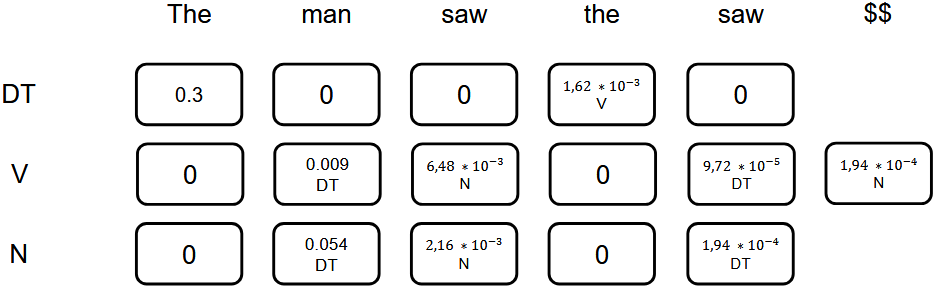
\includegraphics[scale=0.5]{Pics/ViterbiExampleTokenProbabilities.png}
    \caption{Probabilities of each tag for each token}
\end{figure}

\begin{figure}
    [htp]
    \centering
    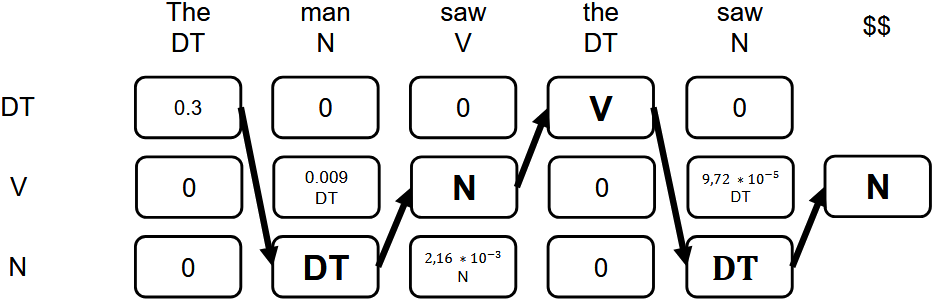
\includegraphics[scale=0.5]{Pics/ViterbiExampleOutput.png}
    \caption{Applied Sequence of tags}
\end{figure}
\end{document}